\subsubsection{CI/CD (Github Action)}

% % CI/CD là
% % phương pháp tự động hóa
% % quy trình tích hợp
% % và triển khai phần mềm.
% % Phương pháp này giúp
% % đẩy nhanh tốc độ, giảm thiểu lỗi thủ công
% % và duy trì độ ổn định cho hệ thống.
% % GitHub Actions là công cụ CI/CD mạnh mẽ được tích hợp sẵn trên GitHub.
% % Trong đồ án này,
% % hệ thống vừa sử dụng Github Action miễn phí của Github,
% % vừa sử dụng Self-hosted runner trên VPS.

% Trong quy trình phát triển phần mềm hiện đại, CI/CD đóng vai trò cốt lõi trong việc tự động hóa quá trình tích hợp và triển khai.

% Phương pháp này giúp
% đẩy nhanh tốc độ, giảm thiểu lỗi thủ công
% và duy trì độ ổn định cho hệ thống.

% Đồ án sử dụng GitHub Actions làm công cụ điều phối CI/CD chính nhờ khả năng tích hợp sẵn trên GitHub.

% Trong đồ án này,
% hệ thống vừa sử dụng Github Action miễn phí của Github (runs-on: ubuntu-latest),
% vừa sử dụng Self-hosted runner trên VPS (runs-on: self-hosted).

Trong quy trình phát triển phần mềm hiện đại,
CI/CD đóng vai trò cốt lõi
trong việc tự động hóa quá trình
tích hợp và triển khai.
Phương pháp này giúp
đẩy nhanh tốc độ,
giảm thiểu lỗi thủ công
và duy trì độ ổn định cho hệ thống.
Đồ án sử dụng GitHub Actions
làm công cụ điều phối CI/CD
nhờ khả năng tích hợp sẵn trên GitHub.
Trong đồ án này,
hệ thống vừa sử dụng Github Action miễn phí
của Github (runs-on: ubuntu-latest),
vừa sử dụng Self-hosted runner
trên VPS (runs-on: self-hosted).

\begin{figure}[H]
\centering
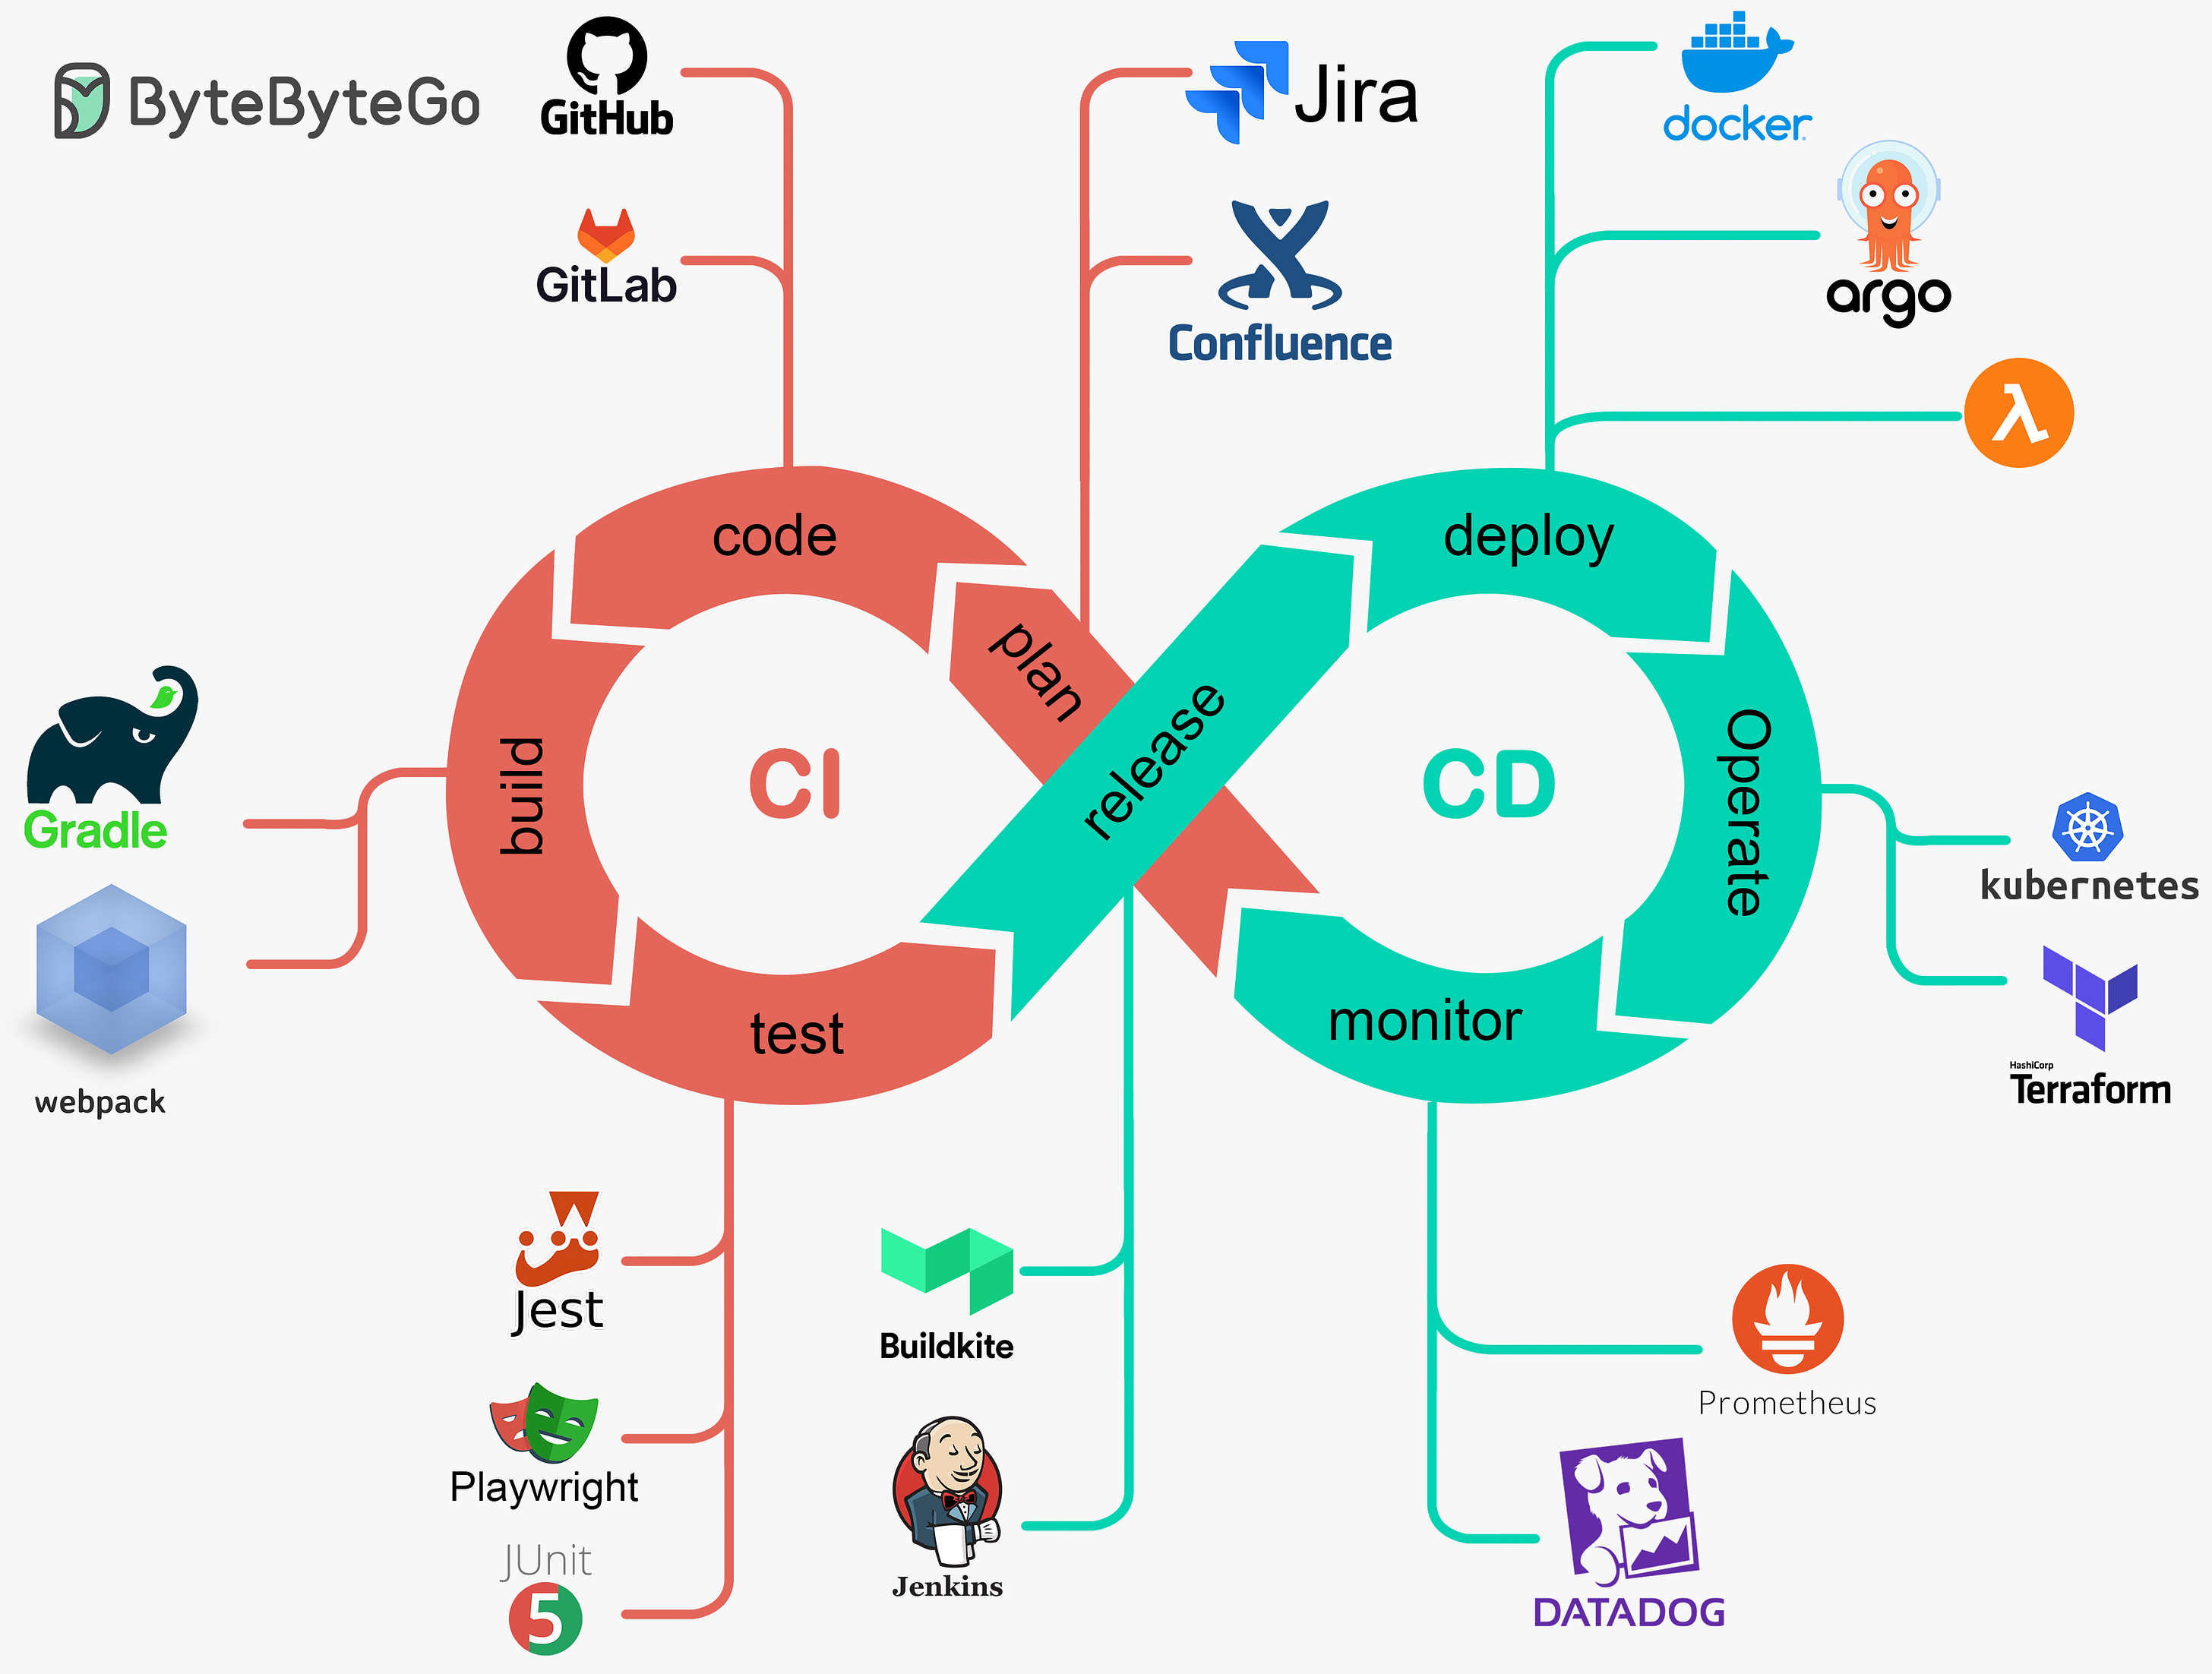
\includegraphics[width=0.98\textwidth]{pictures/cicd-overview.jpg}
\caption[Ví dụ tổng quan CI/CD]{Ví dụ tổng quan CI/CD (Nguồn: \cite{bytebytego-cicd})}
\end{figure}

% \begin{block}{Ứng dụng trong đồ án}

% \end{block}

Sơ đồ tổng quan CI/CD bằng Github Action trong dự án

\begin{figure}[H]
\centering
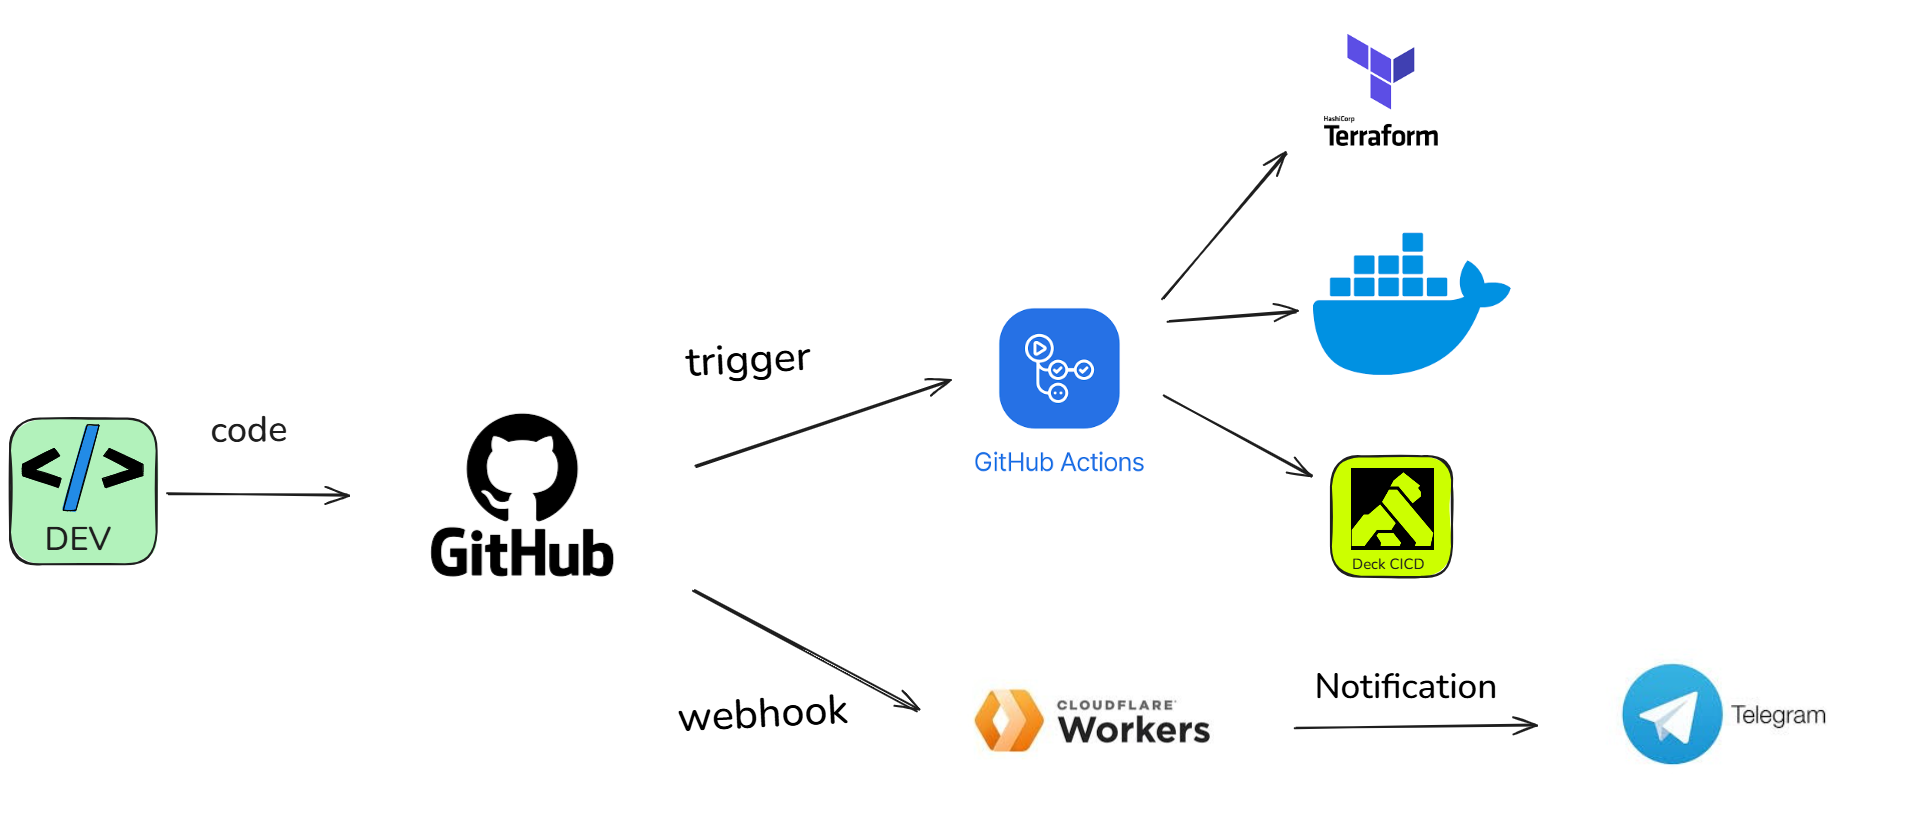
\includegraphics[width=0.98\textwidth]{pictures/cicd-by-github-action.excalidraw.png}
\caption{Sơ đồ tổng quan CI/CD bằng Github Action trong dự án}
\end{figure}
